\documentclass{article}
\usepackage{graphicx}
\usepackage{listings}

\begin{document}

\title{CS 325: Assignment 1}
\author{Jared Wasinger}

\maketitle

 \begin{enumerate}
   \item Intersection of $8n^2$ and $64nlog_2n \approx 43.5593$.  Insertion sort will beat merge sort at $n >= 44$
   \item Table:)
   \item \textbf{Base Case}(n=2):\\
   $2lg2 = 2$\\
   \textbf{Inductive Step}:\\
   $T(2^{k+1}) = 2^{k+1}lg(2^{k+1})$\\
   $T(2^{k+1}) = 2^k*2*lg(2^k*2)$\\
   $T(2^{k+1}) = 2^k*2*lg(2^k)*2lg2$\\
   $T(2^k*2) = 2^k*2*lg(2^k)$\\
   $T(2^k) = 2^k*lg(2^k)$\\
   $T(2^{k+1})$ implies $T(2^k)$\\

   \item Answers:
   \begin{enumerate}
     \item $\lim_{x\to\infty} f(x)/g(x) = \lim_{x\to\infty} n^{0.75}/n^{0.5} = \lim_{x\to\infty} n^{0.25} = \infty$\\
     $f(n) = \Omega(g(n))$

     \item $\lim_{x\to\infty} f(x)/g(x) = \lim_{x\to\infty} \frac{n} {log^2n} = \infty$ (L.H. doesn't simplify result)\\
     $f(n) = \Omega(g(n))$

     \item $\lim_{x\to\infty} f(x)/g(x) = \lim_{x\to\infty} \frac {log(n)} {log_2n} = log(2)$
     $f(n) = \Theta(g(n))$

     \item $\lim_{x\to\infty} f(x)/g(x) = \lim_{x\to\infty} \frac {e^n} {2^n} = \infty$
     $f(n) = \Omega(g(n))$

     \item $\lim_{x\to\infty} f(x)/g(x) = \lim_{x\to\infty} \frac {e^n} {2^n} = \infty$
     $f(n) = \Omega(g(n))$

     \item $\lim_{x\to\infty} f(x)/g(x) = \lim_{x\to\infty} \frac {2^n} {2^n-1} = \lim_{x\to\infty} 2^n-(n-1)=2$
     $f(n) = \Theta(g(n))$

     $f(n) = \Omega(g(n))$
   \end{enumerate}


  \item Algorithm:
    \begin{enumerate}
        \item Split array into pairs of consecutive values
        \item Sort pair elements into local minima maxima (2 arrays): n/2 comparisons
        \item Compare all local minima (associatively) to find global minimum: n/2 comparisons 
        \item Compare all local maxima (associatively) to find global maximum: n/2 comparisons 

     \end{enumerate}
     Worst case performance: 1.5n comparisons\\

     Example: A=[9,3,5,10,1,7,12], n=7
     \begin{enumerate}
       \item (9,3), (5,10), (1,7), (12)
       \item Local Minima: [3,5,1,12], Local Maxima: [9, 10, 7, 12] = 3 comparisons
       \item Global Maximum: 12 = 3 comparisons
       \item Global Minimum: 1 = 3 comparisons 
       \item Total number of comparisons: 9.  9/7 = 1.28n comparisons
     \end{enumerate}
  \item Proofs:
  \item Results:
    \begin{enumerate}
      \item \begin{tabular}{|l|l|l|l|}
        \hline
        \multicolumn{1}{c}{\bfseries n (recursive)} & \multicolumn{1}{c}{\bfseries time (recursive)} & \multicolumn{1}{c}{\bfseries n (iterative)} & \multicolumn{1}{c}{\bfseries time (iterative)} \\ \hline
        10 & 0.01s & 20000 & 0.01s \\ \hline
        15 & 0.01s & 30000 & 0.01s \\ \hline
        20 & 0.01s & 40000 & 0.02s \\ \hline
        30 & 0.26s & 50000 & 0.03s \\ \hline
        35 & 2.89s & 60000 & 0.04s \\ \hline
      \end{tabular}
      \item \textbf{Matplotlib graphing source code}:
      \lstinputlisting{plot.py}
      \textbf{Fibonacci profiling source code}:
      \lstinputlisting{p7.py}
      \item 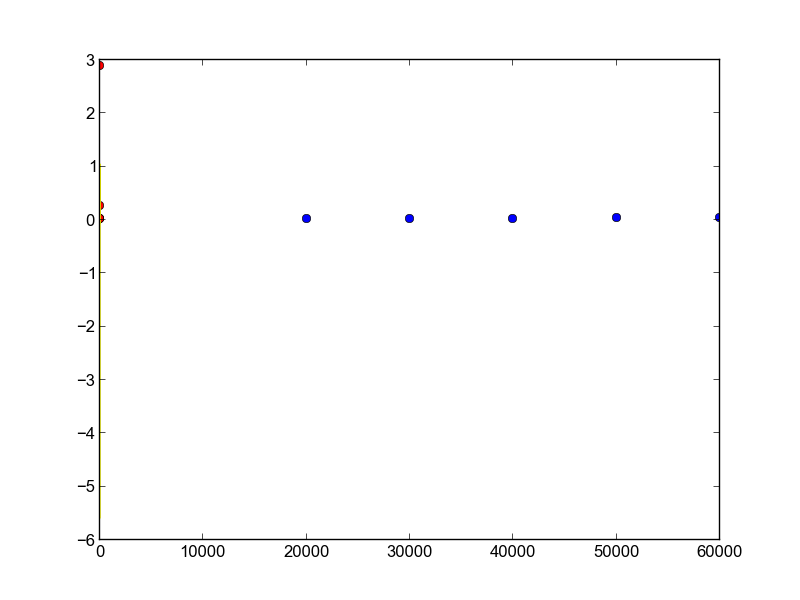
\includegraphics[width=0.8\textwidth]{plot.png}

      \textbf{Polynomial equations of fit}\\
      Polynomial equations are the best fit for these functions because they can be made to approximate the data set to an arbitrary precision.
      \textbf{Recursive fit}: 
      $1.056 \times 10^{-3}x^3 - 6.003 \times 10^-2x^2+ 1.048x - 5.584$\\
      \textbf{Iterative fit}:
      $-8.333 \times 10^{-16}x^3 + 1.143 \times 10^-10x^2 - 4.060\times 10^-6x - 5.20 \times 10^-2$\\
      \textbf{Note}:  These curves of fit do not match the data set.  According to error output I received when running the line-of-fit calculations, this appears to be a numerical error, likely due to the fact that data points are so close to 0.\\
      \item The difference in running times is due to the immense (relative) overhead caused by the recursive implementation of the Fibonacci calculations.  The additional computation cost imposed by recursive function calls (call stack manipulation) is very restrictive.

    \end{enumerate}

\end{enumerate}
\end{document}
